\documentclass[tikz,border=3pt]{standalone}
\usepackage[T1]{fontenc}
\usepackage{helvet}
\renewcommand{\familydefault}{\sfdefault}
\usepackage{setspace}
\usetikzlibrary{positioning,arrows.meta,shapes.geometric}

\begin{document}
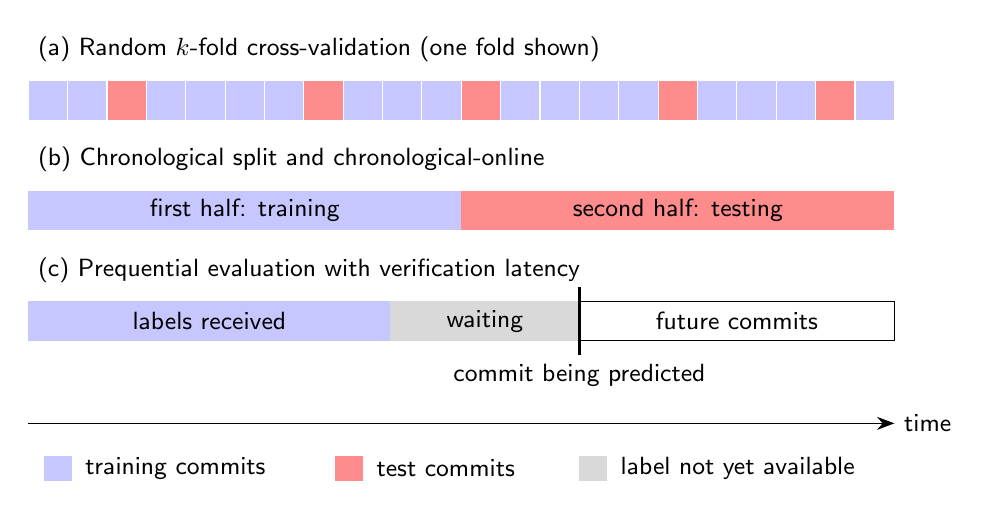
\begin{tikzpicture}[font=\small, x=1cm, y=1cm]
\def\w{11}
\node[anchor=west] at (0,5.6) {(a) Random $k$-fold cross-validation (one fold shown)};
\foreach \i in {0,...,21} {
  \pgfmathtruncatemacro{\istest}{(\i==2 || \i==7 || \i==11 || \i==16 || \i==20) ? 1 : 0}
  \ifnum\istest=1
    \fill[red!45] (\i*0.5,4.7) rectangle ++(0.5,0.5);
  \else
    \fill[blue!22] (\i*0.5,4.7) rectangle ++(0.5,0.5);
  \fi
  \draw[white] (\i*0.5,4.7) rectangle ++(0.5,0.5);
}
\node[anchor=west] at (0,4.2) {(b) Chronological split and chronological-online};
\fill[blue!22] (0,3.3) rectangle (5.5,3.8);
\fill[red!45] (5.5,3.3) rectangle (\w,3.8);
\node at (2.75,3.55) {first half: training};
\node at (8.25,3.55) {second half: testing};
\node[anchor=west] at (0,2.8) {(c) Prequential evaluation with verification latency};
\fill[blue!22] (0,1.9) rectangle (4.6,2.4);
\fill[gray!30] (4.6,1.9) rectangle (7.0,2.4);
\draw (7.0,1.9) rectangle (\w,2.4);
\draw[thick] (7.0,1.72) -- (7.0,2.58);
\node at (2.3,2.15) {labels received};
\node at (5.8,2.15) {waiting};
\node at (9.0,2.15) {future commits};
\node[anchor=north] at (7.0,1.72) {commit being predicted};
\draw[-{Stealth[length=2.2mm]}] (0,0.85) -- (\w,0.85) node[right] {time};
\fill[blue!22] (0.2,0.12) rectangle ++(0.35,0.32); \node[anchor=west] at (0.6,0.28) {training commits};
\fill[red!45] (3.9,0.12) rectangle ++(0.35,0.32); \node[anchor=west] at (4.3,0.28) {test commits};
\fill[gray!30] (7.0,0.12) rectangle ++(0.35,0.32); \node[anchor=west] at (7.4,0.28) {label not yet available};
\end{tikzpicture}
\end{document}
